\subsection{Syntax units}
\label{sec:syntax-units}
We saw how the input and forget gate of number units control the flow
of subject number information. It remains unclear, however, how are
the dynamics of these gates controlled by the network. We hypothesized
that other units may encode information about the syntactic structure
of the sentence, and in particular, about the subject-verb
dependency. To explore this, we tested whether syntactic information
can be decoded from other units in the network, by using the depth of
the syntactic tree as a proxy \cite{Nelson:etal:2017}. Specifically,
we trained an L2-regularized regression models to predict
syntactic tree-depth from the hidden-state activity of all units,
using the data presented in Section \ref{sec:the_data} above in nested
5-fold cross-validation (CV) procedure (the optimal regularization size was found to be consistent across CV-splits, $\lambda=784.76$, among 20 possible values log-uniformly distributed in $[10^-5, 10^5]$ \yair{add regularization plots to SOM?}). Word position and tree-depth were decorrelated in the data and word frequency was added as a covariate
to the model and had a negligable effect on the results.

Syntactic tree-depth can be efficiently decoded from network activity
($R^2_{test-set}=0.85\pm0.009$; covariate corrected). A small subset of units we will refer to
as `syntax units' had relatively high weights in the regression model (mean weight = $7.6*10^{-4}$, standard deviation(SD)=$7.86*10^{-2}$; cutoff for outlier weights was set to three SDs)\yair{Discuss issues with interpreting weights}. The syntax
units, as a set, were found to be crucial for accomplishing the NA-task, since
ablating them resulted in significant performance reduction in several NA-tasks compared
to 1000 random ablations of subsets of units of the same size
(Linzen NA-task: $p-value=0.024$, nounPP-SP: $p-value=$, nounPP-PS: $p-value=$ \yair{complete: report ablation results from all NA-tasks}).\marco{I would add the accuracy when ablating the two number units in the
  plot, and, as I expect this to be larger, discuss the fact that
  probably what we identified here is not the complete syntax-tracking
  sub-network.}

%\begin{figure}[h]
%    \centering
%    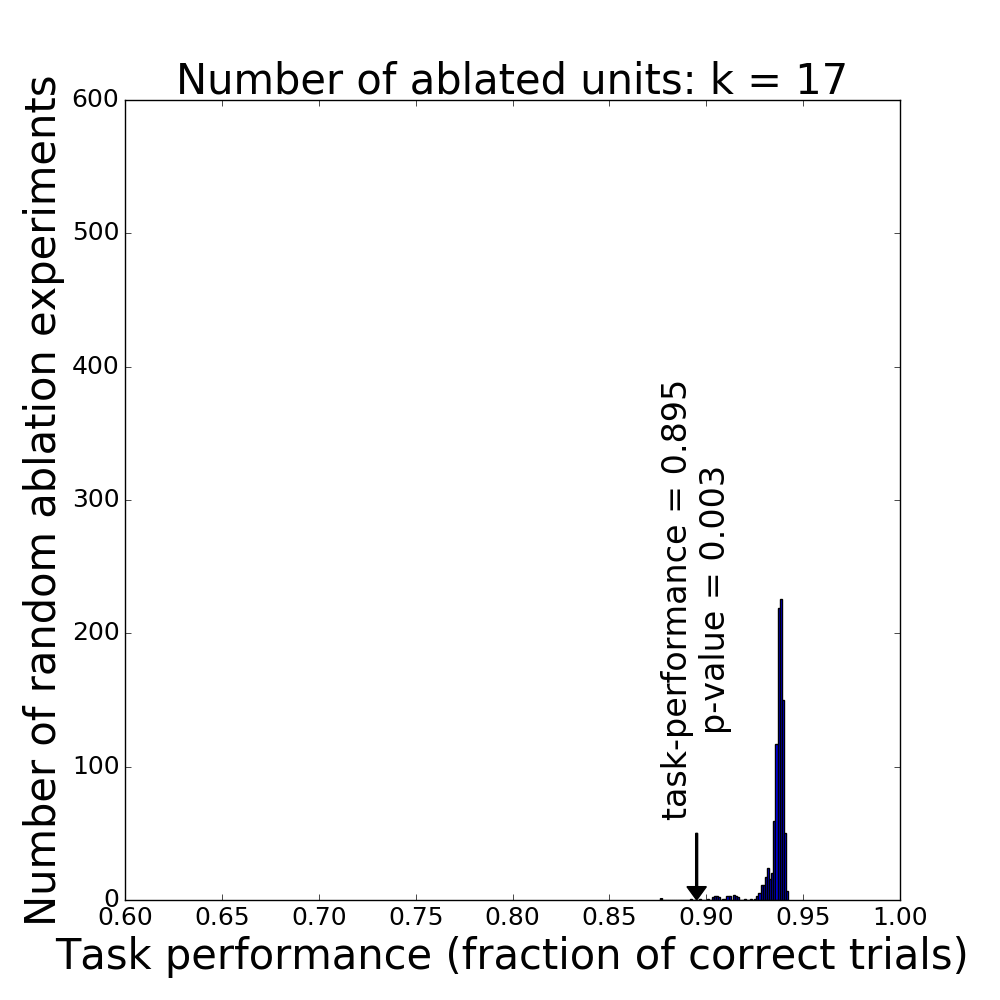
\includegraphics[height=5cm]{Figures/null_distribution_ablation_experiment_k_17.png}
%    \caption{Distribution of NA-tasks accuracy when ablating 17 units,
%      either random (N=1000) or the syntax units (downward arrow).}
%    \label{fig:ablation-syntax}
%\end{figure}

\begin{figure*}[t]
    \begin{subfigure}{0.32\textwidth}
            \centering
            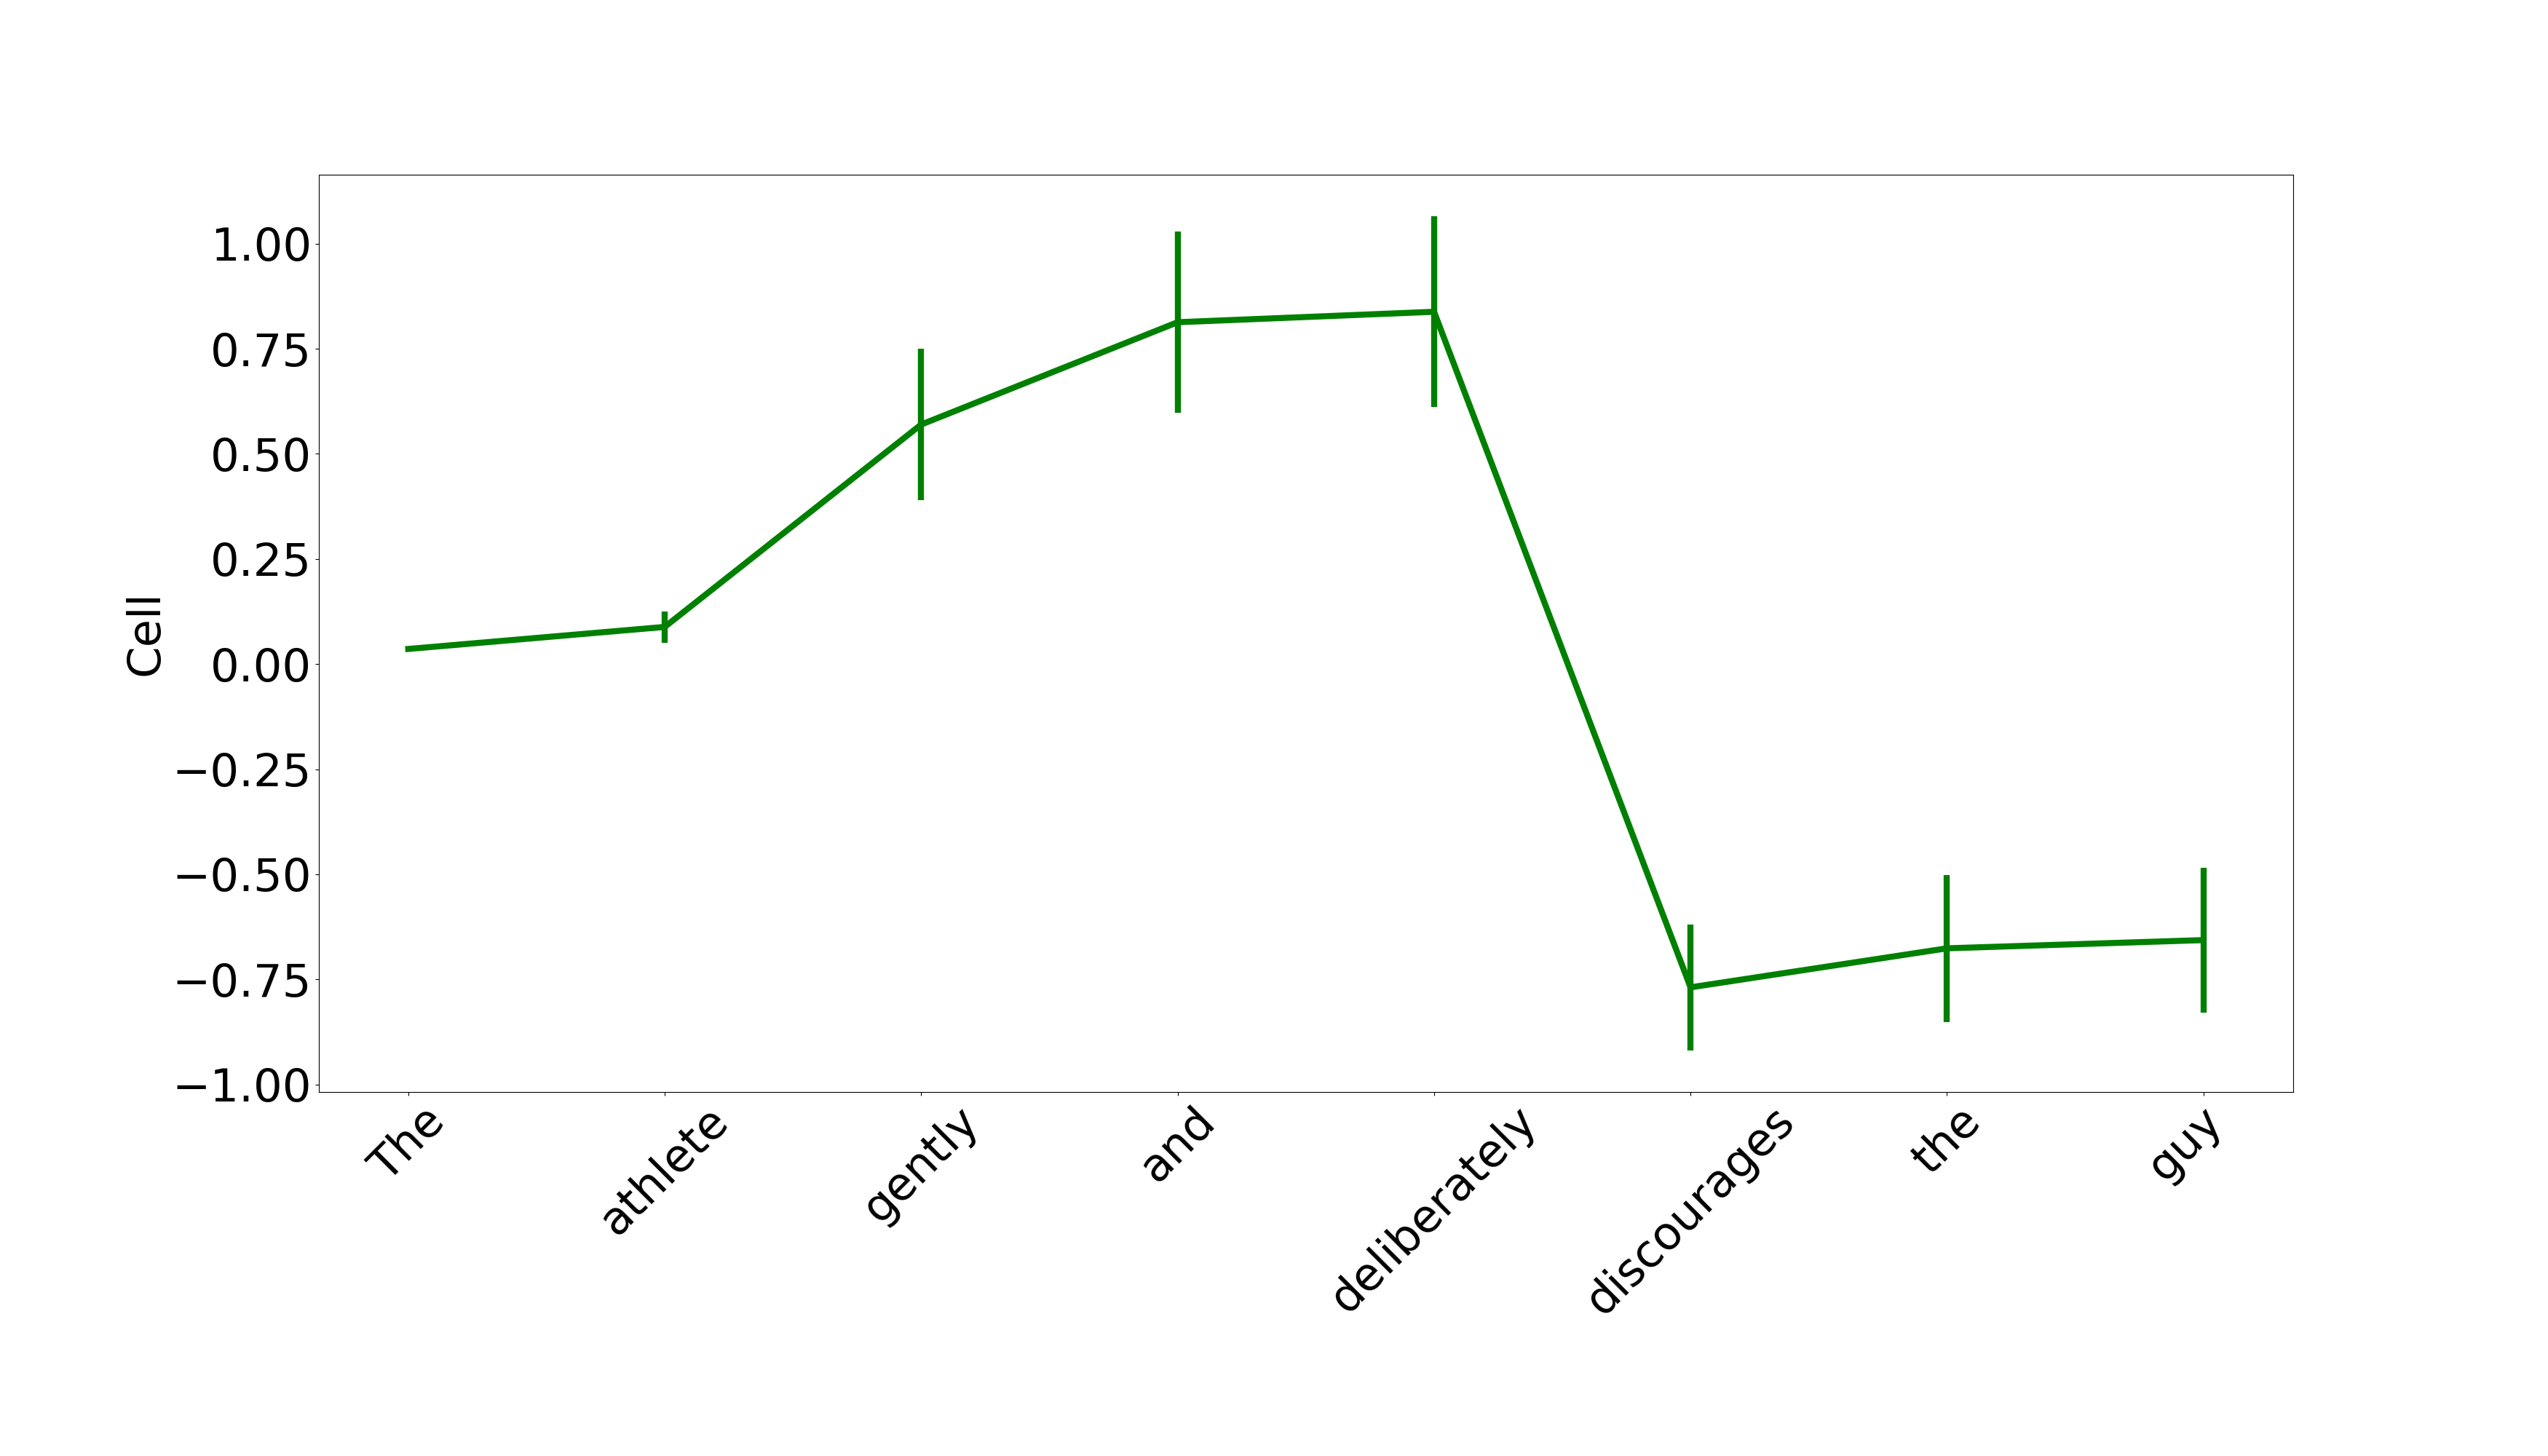
\includegraphics[width=\linewidth, height=3cm]{Figures/adv_conjunction_1149_cell}
            \caption{2Adv}
            \label{fig:syntax-unit-2Adv}
    \end{subfigure}
    \begin{subfigure}{0.32\textwidth}
            \centering
            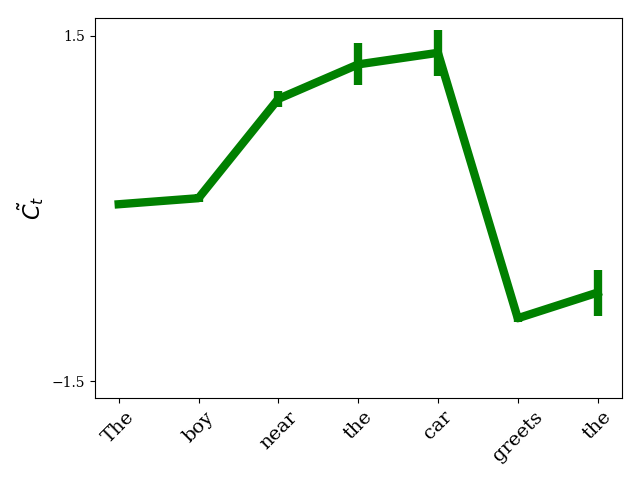
\includegraphics[width=\linewidth, height=3cm]{Figures/nounpp_1149_cell.png}
            \caption{nounPP}
            \label{fig:syntax-unit-nounpp}
    \end{subfigure}
    \begin{subfigure}{0.32\textwidth}
            \centering
            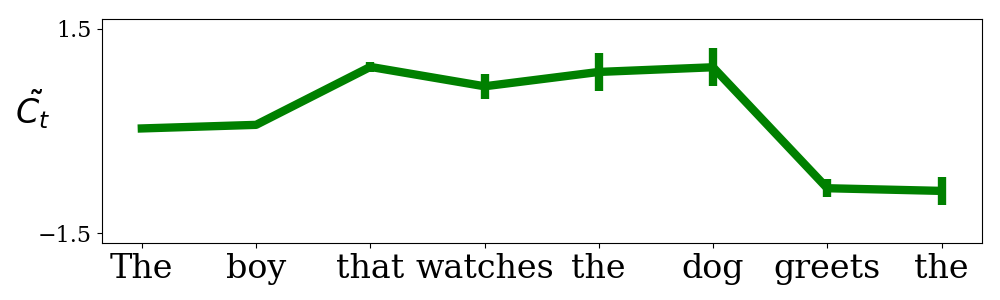
\includegraphics[width=\linewidth, height=3cm]{Figures/subjrel_that_1149_cell.png}
            \caption{subject relative}
            \label{fig:syntax-unit-subjrel}
    \end{subfigure}
    \begin{subfigure}{\textwidth}
            \centering
            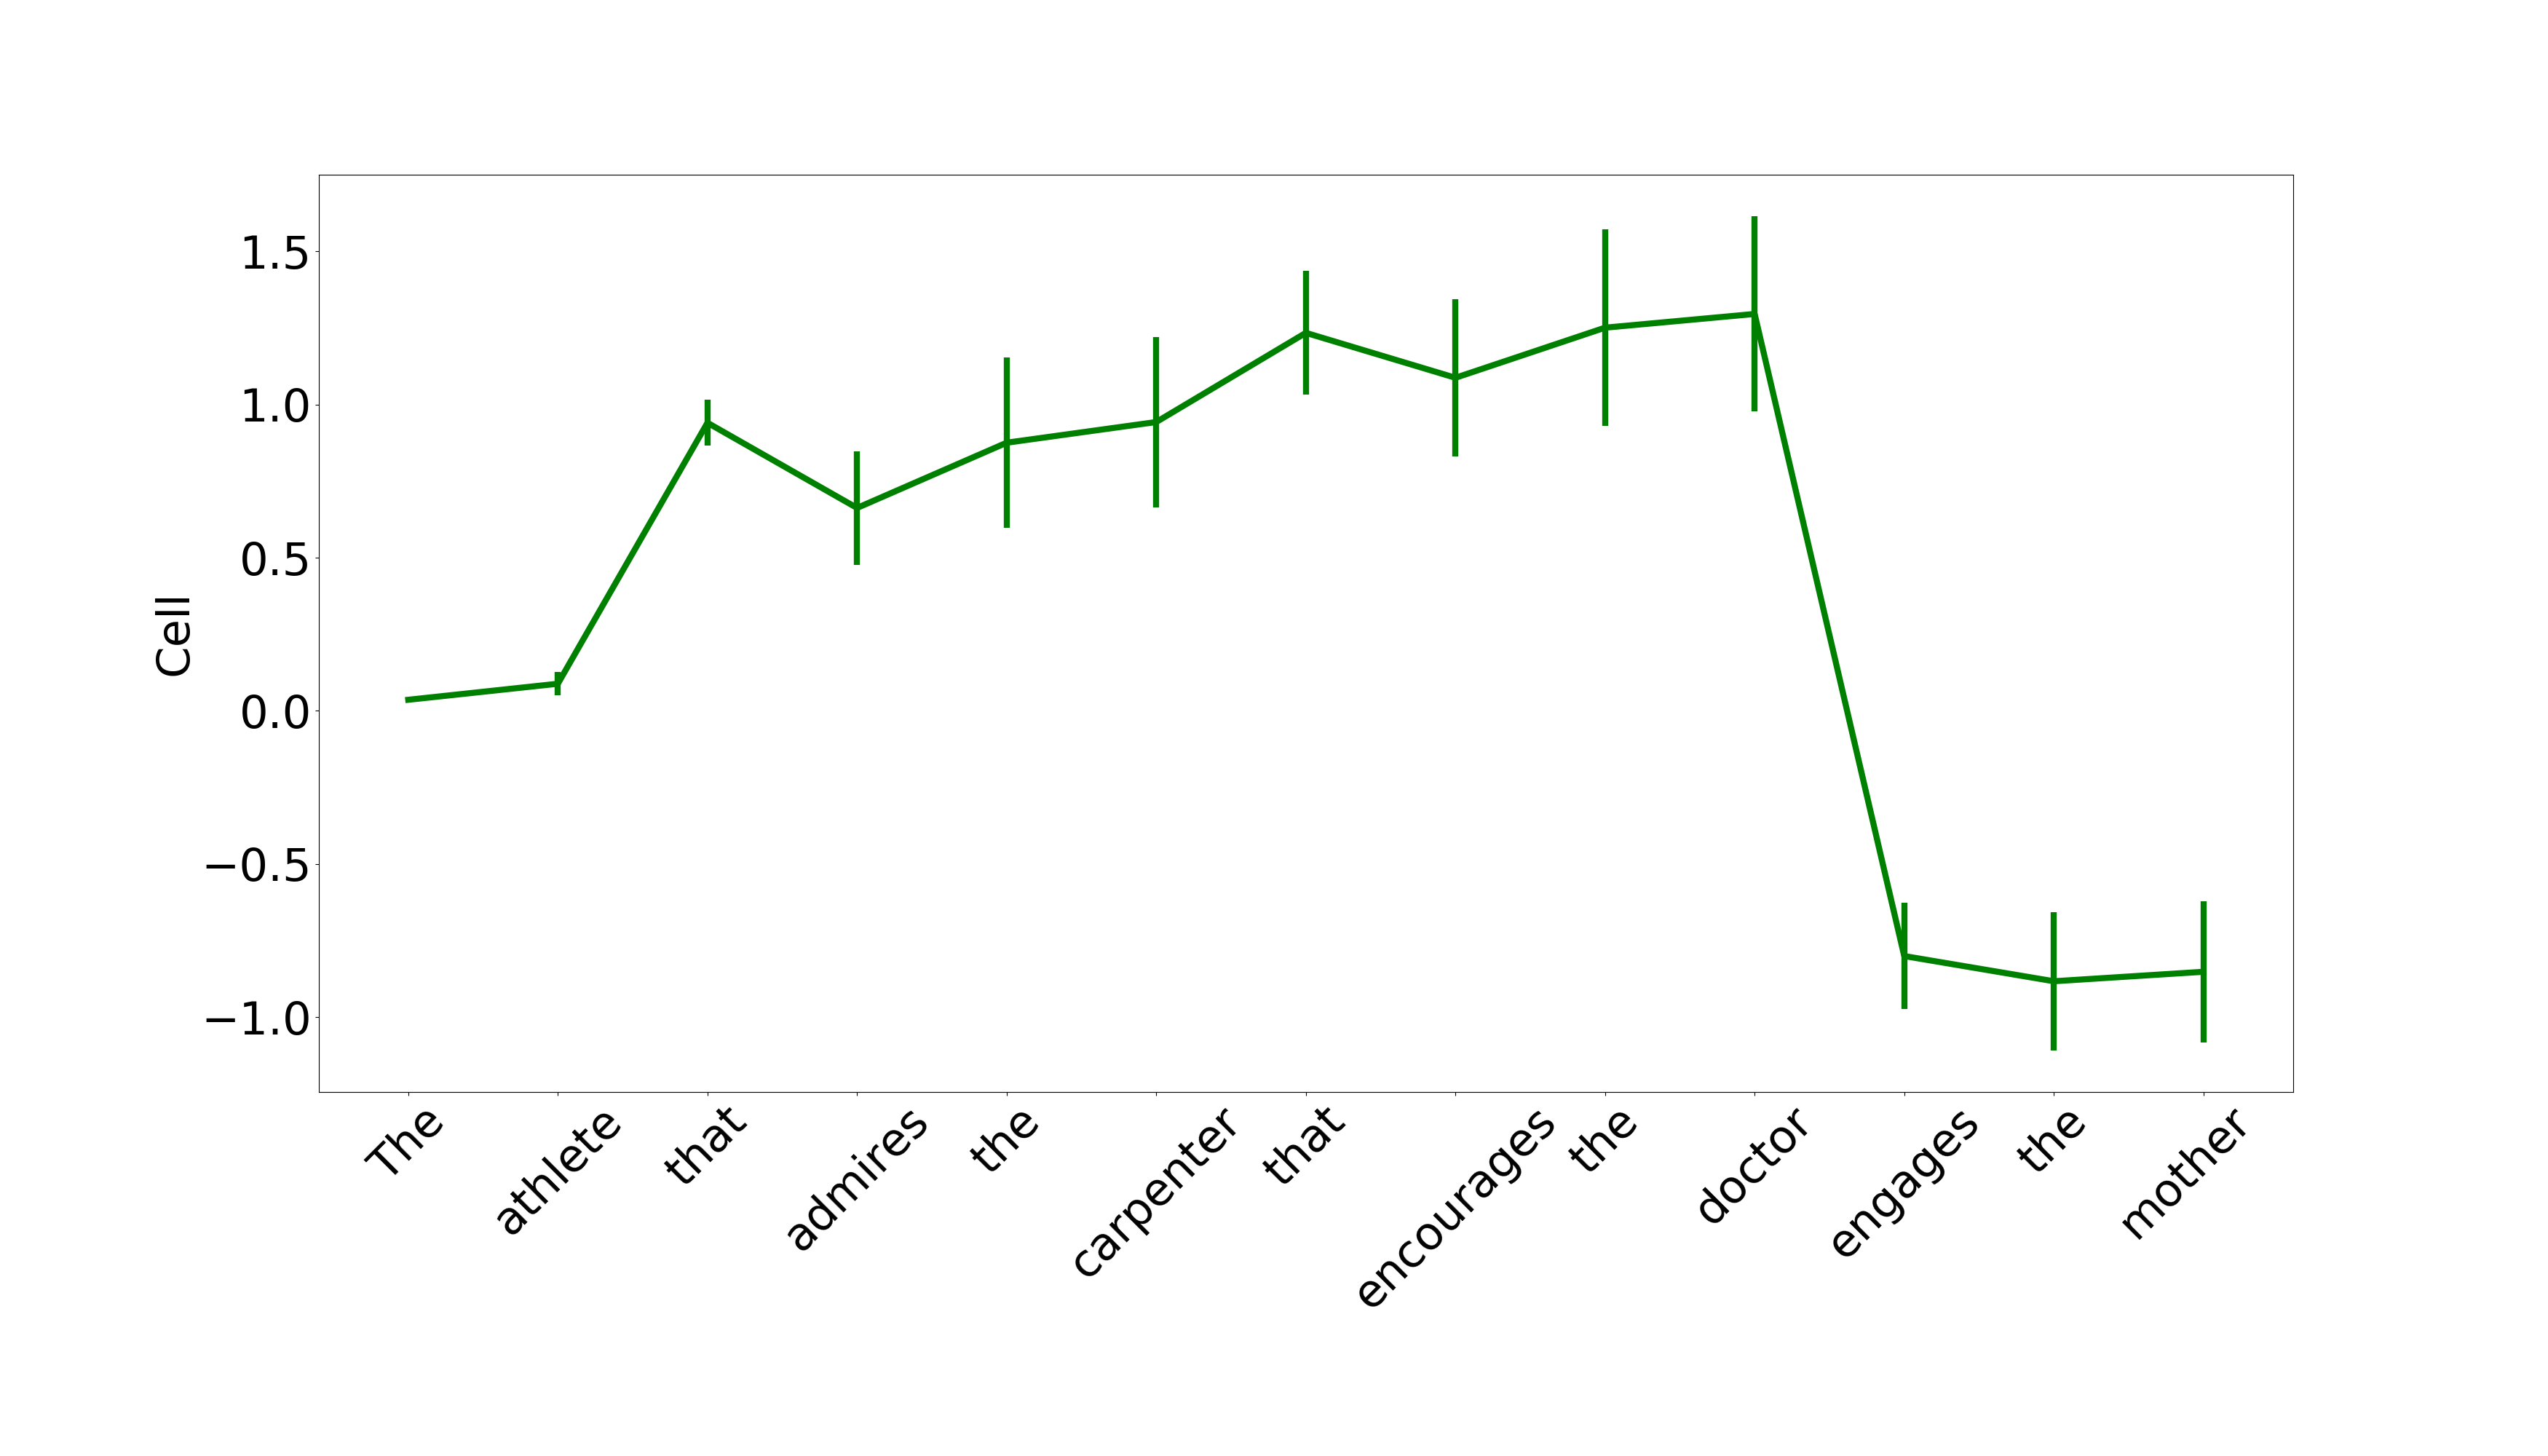
\includegraphics[width=\linewidth, height=3cm]{Figures/double_subjrel_that_1149_cell.png}
            \caption{Two embeddings with subject relatives}
            \label{fig:syntax-unit-double-subjrel}
    \end{subfigure}
\caption{Cell activity of syntax unit \unit{2}{500} while processing various syntactic structures. Error bars represent standard deviations across all stimuli. \yair{improve visualization}}
\end{figure*}

We next looked into the dynamics of the syntax units by visualizing
their gate and cell dynamics during sentence processing. We found that
cell activity of one of them, unit \unit{2}{500},
which also had the highest weight in the regression model above, was
remarkably structured. Cell activity of this unit was found to
increase across the entire subject-verb dependency and to abruptly
drop right after. Figures \ref{fig:syntax-unit-2Adv} and
\ref{fig:syntax-unit-nounpp} show cell activity of this unit during
the processing of stimuli from the 2Adv and nounPP tasks. We found the
same dynamics in cases where another verb occurs between subject and
main verb, as in subject relatives (Figure
\ref{fig:syntax-unit-subjrel}), and in exceptionally long-distance
dependencies with two interfering nouns and verbs (Figure
\ref{fig:syntax-unit-double-subjrel}). Taken together, these results
suggest that unit \unit{2}{500} consistently encodes
subject-verb dependency in a syntax-sensitive manner. 
\footnote{Other syntax units did not show an easily interpretable
  dynamics, nor clear interactions with the number units, as shown below, but\ldots}

